\documentclass{article}\usepackage[]{graphicx}\usepackage[]{color}
% maxwidth is the original width if it is less than linewidth
% otherwise use linewidth (to make sure the graphics do not exceed the margin)
\makeatletter
\def\maxwidth{ %
  \ifdim\Gin@nat@width>\linewidth
    \linewidth
  \else
    \Gin@nat@width
  \fi
}
\makeatother

\definecolor{fgcolor}{rgb}{0.345, 0.345, 0.345}
\newcommand{\hlnum}[1]{\textcolor[rgb]{0.686,0.059,0.569}{#1}}%
\newcommand{\hlstr}[1]{\textcolor[rgb]{0.192,0.494,0.8}{#1}}%
\newcommand{\hlcom}[1]{\textcolor[rgb]{0.678,0.584,0.686}{\textit{#1}}}%
\newcommand{\hlopt}[1]{\textcolor[rgb]{0,0,0}{#1}}%
\newcommand{\hlstd}[1]{\textcolor[rgb]{0.345,0.345,0.345}{#1}}%
\newcommand{\hlkwa}[1]{\textcolor[rgb]{0.161,0.373,0.58}{\textbf{#1}}}%
\newcommand{\hlkwb}[1]{\textcolor[rgb]{0.69,0.353,0.396}{#1}}%
\newcommand{\hlkwc}[1]{\textcolor[rgb]{0.333,0.667,0.333}{#1}}%
\newcommand{\hlkwd}[1]{\textcolor[rgb]{0.737,0.353,0.396}{\textbf{#1}}}%
\let\hlipl\hlkwb

\usepackage{framed}
\makeatletter
\newenvironment{kframe}{%
 \def\at@end@of@kframe{}%
 \ifinner\ifhmode%
  \def\at@end@of@kframe{\end{minipage}}%
  \begin{minipage}{\columnwidth}%
 \fi\fi%
 \def\FrameCommand##1{\hskip\@totalleftmargin \hskip-\fboxsep
 \colorbox{shadecolor}{##1}\hskip-\fboxsep
     % There is no \\@totalrightmargin, so:
     \hskip-\linewidth \hskip-\@totalleftmargin \hskip\columnwidth}%
 \MakeFramed {\advance\hsize-\width
   \@totalleftmargin\z@ \linewidth\hsize
   \@setminipage}}%
 {\par\unskip\endMakeFramed%
 \at@end@of@kframe}
\makeatother

\definecolor{shadecolor}{rgb}{.97, .97, .97}
\definecolor{messagecolor}{rgb}{0, 0, 0}
\definecolor{warningcolor}{rgb}{1, 0, 1}
\definecolor{errorcolor}{rgb}{1, 0, 0}
\newenvironment{knitrout}{}{} % an empty environment to be redefined in TeX

\usepackage{alltt}

\usepackage{float}

% Set the margins on the page to not be so large
\addtolength{\oddsidemargin}{-.875in}
\addtolength{\evensidemargin}{-.875in}
\addtolength{\textwidth}{1.75in}
\addtolength{\topmargin}{-.875in}
\addtolength{\textheight}{1.75in}

% Take off page numbering
\pagenumbering{gobble}
\IfFileExists{upquote.sty}{\usepackage{upquote}}{}
\begin{document}

\title{%
  4.3.1: R - Nonparametric Regression Methods \\
  (LOESS, Regression Trees, and Random Forests)
  \smallskip
  \large Stat 5100: Dr. Bean
}
\date{}

\maketitle

\textbf{Example: } Baseball dataset (same as Handout 4.1.1)

\begin{knitrout}
\definecolor{shadecolor}{rgb}{0.969, 0.969, 0.969}\color{fgcolor}\begin{kframe}
\begin{alltt}
\hlkwd{library}\hlstd{(stat5100)}
\hlkwd{data}\hlstd{(baseball)}
\hlkwd{head}\hlstd{(baseball)}
\end{alltt}
\begin{verbatim}
##                Name      Team nAtBat nHits nHome nRuns nRBI nBB YrMajor CrAtBat
## 1    Allanson, Andy Cleveland    293    66     1    30   29  14       1     293
## 2       Ashby, Alan   Houston    315    81     7    24   38  39      14    3449
## 3       Davis, Alan   Seattle    479   130    18    66   72  76       3    1624
## 4     Dawson, Andre  Montreal    496   141    20    65   78  37      11    5628
## 5 Galarraga, Andres  Montreal    321    87    10    39   42  30       2     396
## 6  Griffin, Alfredo   Oakland    594   169     4    74   51  35      11    4408
##   CrHits CrHome CrRuns CrRbi CrBB   League Division Position nOuts nAssts
## 1     66      1     30    29   14 American     East        C   446     33
## 2    835     69    321   414  375 National     West        C   632     43
## 3    457     63    224   266  263 American     West       1B   880     82
## 4   1575    225    828   838  354 National     East       RF   200     11
## 5    101     12     48    46   33 National     East       1B   805     40
## 6   1133     19    501   336  194 American     West       SS   282    421
##   nError Salary Div logSalary
## 1     20     NA  AE        NA
## 2     10  475.0  NW  6.163315
## 3     14  480.0  AW  6.173786
## 4      3  500.0  NE  6.214608
## 5      4   91.5  NE  4.516339
## 6     25  750.0  AW  6.620073
\end{verbatim}
\end{kframe}
\end{knitrout}

\subsection*{LOESS Regression}

\begin{knitrout}
\definecolor{shadecolor}{rgb}{0.969, 0.969, 0.969}\color{fgcolor}\begin{kframe}
\begin{alltt}
\hlstd{baseball_loess} \hlkwb{<-} \hlkwd{loess}\hlstd{(logSalary} \hlopt{~} \hlstd{CrAtBat} \hlopt{+} \hlstd{nBB,} \hlkwc{data} \hlstd{= baseball,}
                        \hlkwc{degree} \hlstd{=} \hlnum{2}\hlstd{,} \hlkwc{span} \hlstd{=} \hlnum{0.6}\hlstd{)}

\hlstd{crAtBat_range} \hlkwb{<-} \hlkwd{seq}\hlstd{(}\hlkwd{min}\hlstd{(baseball}\hlopt{$}\hlstd{CrAtBat),} \hlkwd{max}\hlstd{(baseball}\hlopt{$}\hlstd{CrAtBat),} \hlkwc{length} \hlstd{=} \hlnum{500}\hlstd{)}
\hlstd{nBB_range} \hlkwb{<-} \hlkwd{seq}\hlstd{(}\hlkwd{min}\hlstd{(baseball}\hlopt{$}\hlstd{nBB),} \hlkwd{max}\hlstd{(baseball}\hlopt{$}\hlstd{nBB),} \hlkwc{length} \hlstd{=} \hlnum{500}\hlstd{)}
\hlstd{loess_pred} \hlkwb{<-} \hlkwa{function}\hlstd{(}\hlkwc{x}\hlstd{,} \hlkwc{y}\hlstd{) \{}
  \hlkwd{predict}\hlstd{(baseball_loess,} \hlkwd{data.frame}\hlstd{(}\hlkwc{CrAtBat} \hlstd{= x,}
                                     \hlkwc{nBB} \hlstd{= y))}
\hlstd{\}}

\hlstd{z} \hlkwb{<-} \hlkwd{outer}\hlstd{(crAtBat_range, nBB_range, loess_pred)}

\hlcom{# plotly::plot_ly(}
\hlcom{#   x = crAtBat_range,}
\hlcom{#   y = nBB_range,}
\hlcom{#   z = outer(crAtBat_range, nBB_range, loess_pred),}
\hlcom{#   trace = "contour"}
\hlcom{# )}
\end{alltt}
\end{kframe}
\end{knitrout}

\newpage

\subsection*{Regression Trees}

\begin{knitrout}
\definecolor{shadecolor}{rgb}{0.969, 0.969, 0.969}\color{fgcolor}\begin{kframe}
\begin{alltt}
\hlcom{# Fit a regression tree model on the baseball dataset with controls}
\hlstd{baseball_rtree_control} \hlkwb{<-} \hlstd{rpart}\hlopt{::}\hlkwd{rpart.control}\hlstd{(}\hlkwc{maxdepth} \hlstd{=} \hlnum{15}\hlstd{)}
\hlstd{baseball_rtree} \hlkwb{<-} \hlstd{rpart}\hlopt{::}\hlkwd{rpart}\hlstd{(logSalary} \hlopt{~} \hlstd{nAtBat} \hlopt{+} \hlstd{nHits} \hlopt{+} \hlstd{nHome} \hlopt{+} \hlstd{nRuns} \hlopt{+}
                                 \hlstd{nRBI} \hlopt{+} \hlstd{nBB} \hlopt{+} \hlstd{YrMajor} \hlopt{+} \hlstd{CrAtBat} \hlopt{+} \hlstd{CrHits} \hlopt{+}
                                 \hlstd{CrHome} \hlopt{+} \hlstd{CrRuns} \hlopt{+} \hlstd{CrRbi} \hlopt{+} \hlstd{CrBB} \hlopt{+} \hlstd{League} \hlopt{+}
                                 \hlstd{Division} \hlopt{+} \hlstd{nOuts} \hlopt{+} \hlstd{nAssts} \hlopt{+} \hlstd{nError,}
                               \hlkwc{data} \hlstd{= baseball,} \hlkwc{control} \hlstd{= baseball_rtree_control)}

\hlcom{# Look at cost-complexity analysis plot (can help you decide on amount}
\hlcom{# of pruning in your tree)}
\hlstd{rpart}\hlopt{::}\hlkwd{plotcp}\hlstd{(baseball_rtree)}
\end{alltt}
\end{kframe}

{\centering 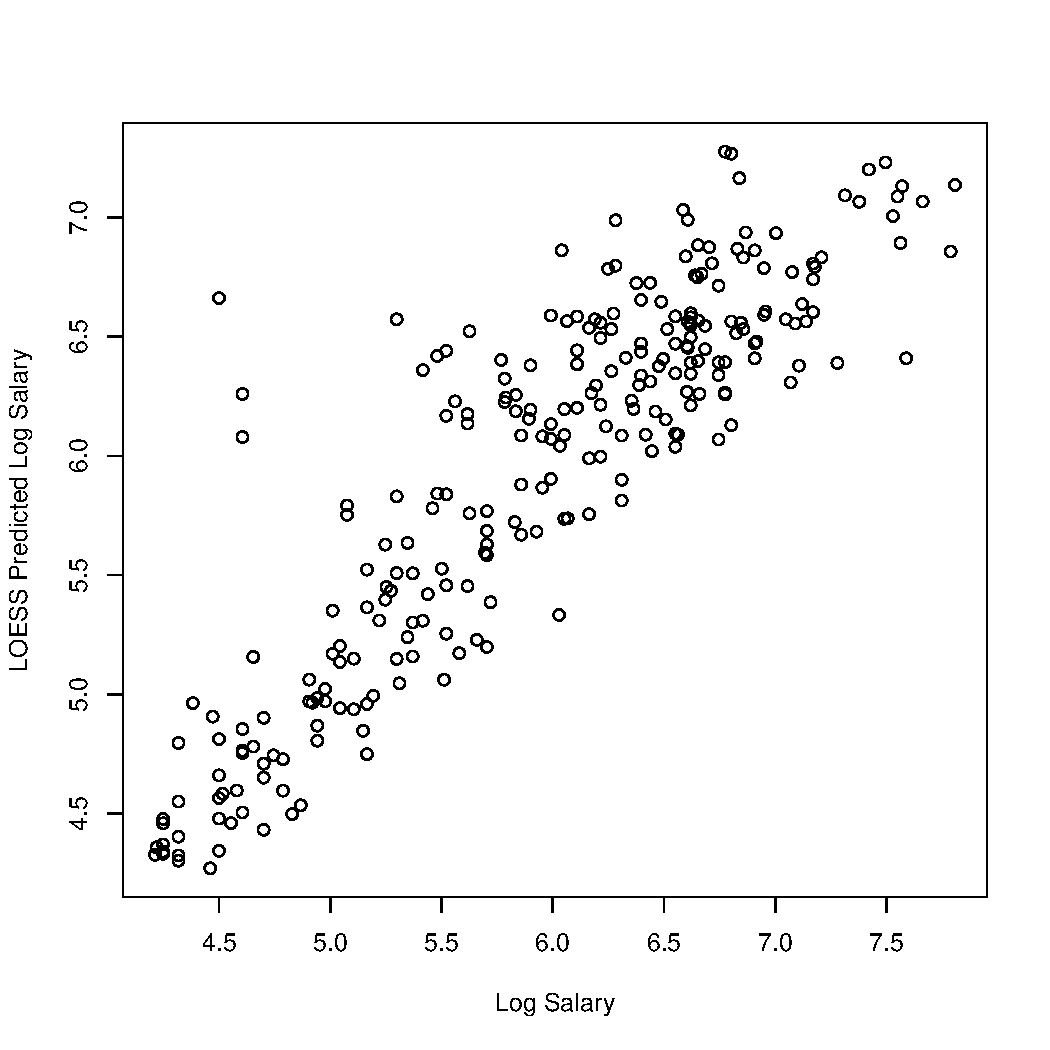
\includegraphics[width=0.6\textwidth]{figure/unnamed-chunk-3-1} 

}



\end{knitrout}

Based upon the above plot, we would likely choose a value of $cp = 0.03$, but we could also go with $cp = 0.022$. Using this value, we can retrain our regression tree model but with more pruning (specified with $cp$).

\begin{knitrout}
\definecolor{shadecolor}{rgb}{0.969, 0.969, 0.969}\color{fgcolor}\begin{kframe}
\begin{alltt}
\hlcom{# Specify a cp=0.03 value for this regression tree model based upon the above plot.}
\hlstd{baseball_final_rtree} \hlkwb{<-}\hlstd{rpart}\hlopt{::}\hlkwd{rpart}\hlstd{(logSalary} \hlopt{~} \hlstd{nAtBat} \hlopt{+} \hlstd{nHits} \hlopt{+} \hlstd{nHome} \hlopt{+} \hlstd{nRuns} \hlopt{+}
                                      \hlstd{nRBI} \hlopt{+} \hlstd{nBB} \hlopt{+} \hlstd{YrMajor} \hlopt{+} \hlstd{CrAtBat} \hlopt{+} \hlstd{CrHits} \hlopt{+}
                                      \hlstd{CrHome} \hlopt{+} \hlstd{CrRuns} \hlopt{+} \hlstd{CrRbi} \hlopt{+} \hlstd{CrBB} \hlopt{+} \hlstd{League} \hlopt{+}
                                      \hlstd{Division} \hlopt{+} \hlstd{nOuts} \hlopt{+} \hlstd{nAssts} \hlopt{+} \hlstd{nError,}
                               \hlkwc{data} \hlstd{= baseball,} \hlkwc{cp} \hlstd{=} \hlnum{0.03}\hlstd{,}
                               \hlkwc{control} \hlstd{= baseball_rtree_control)}
\hlstd{rpart.plot}\hlopt{::}\hlkwd{rpart.plot}\hlstd{(baseball_final_rtree)}
\end{alltt}
\end{kframe}

{\centering 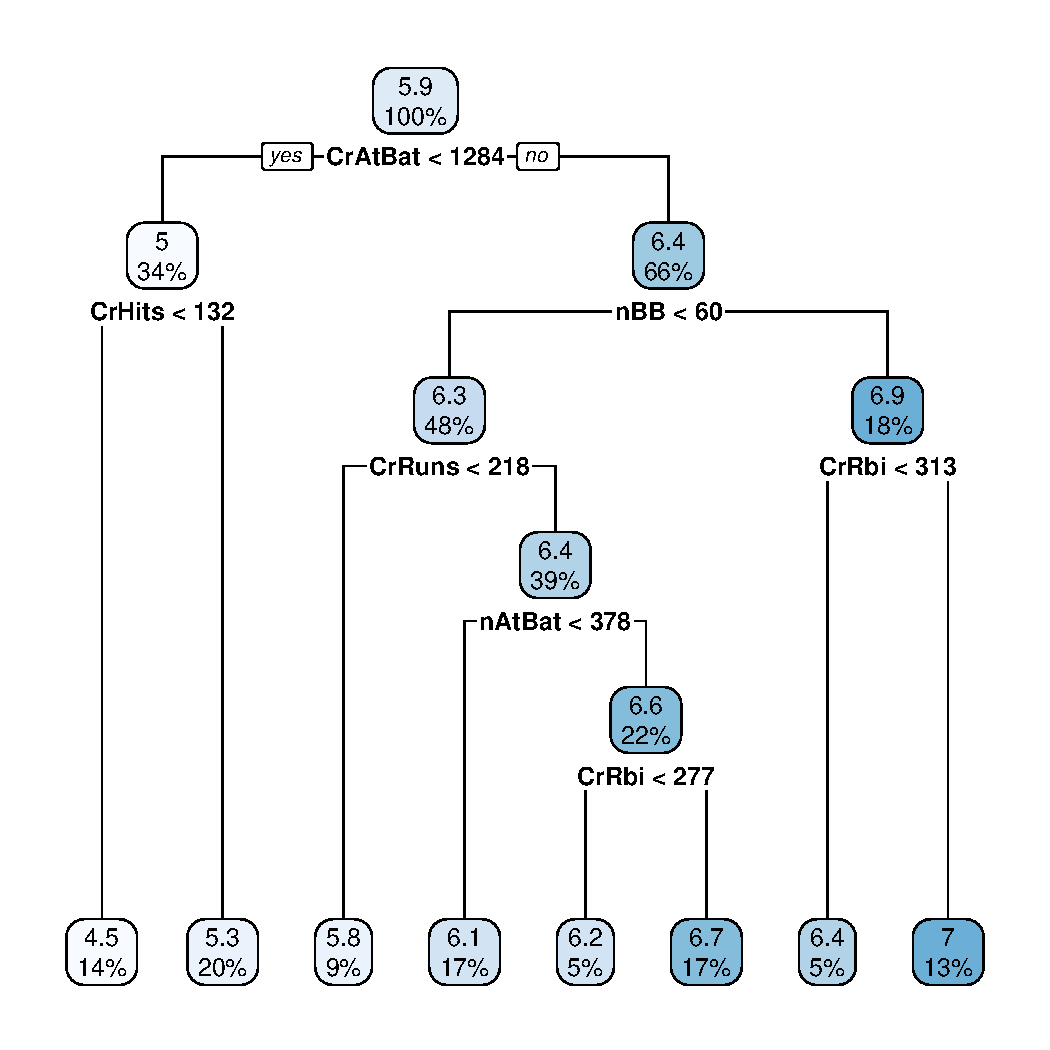
\includegraphics[width=0.6\textwidth]{figure/unnamed-chunk-4-1} 

}



\end{knitrout}

We can also look at the importance of various predictor variables. Note that in the following plot, the higher numbers correspond to more important variables.

\begin{knitrout}
\definecolor{shadecolor}{rgb}{0.969, 0.969, 0.969}\color{fgcolor}\begin{kframe}
\begin{alltt}
\hlstd{baseball_final_rtree}\hlopt{$}\hlstd{variable.importance}
\end{alltt}
\begin{verbatim}
##    CrAtBat     CrHits     CrRuns      CrRbi       CrBB    YrMajor        nBB 
## 146.324332 141.326029 135.892077 124.933828 114.069502  81.776124  15.722008 
##     CrHome      nRuns     nAtBat      nHits       nRBI      nOuts      nHome 
##   9.306841   8.082672   5.981392   5.437629   4.078222   2.446933   1.106655
\end{verbatim}
\end{kframe}
\end{knitrout}

Check out this plot of the known value of logSalary and predicted logSalary:

\begin{knitrout}
\definecolor{shadecolor}{rgb}{0.969, 0.969, 0.969}\color{fgcolor}\begin{kframe}
\begin{alltt}
\hlstd{pred_baseball_logSalary} \hlkwb{<-} \hlkwd{predict}\hlstd{(baseball_final_rtree, baseball)}
\hlkwd{plot}\hlstd{(baseball}\hlopt{$}\hlstd{logSalary, pred_baseball_logSalary,} \hlkwc{xlab} \hlstd{=} \hlstr{"Log Salary"}\hlstd{,}
     \hlkwc{ylab} \hlstd{=} \hlstr{"Predicted logSalary"}\hlstd{)}
\end{alltt}
\end{kframe}

{\centering 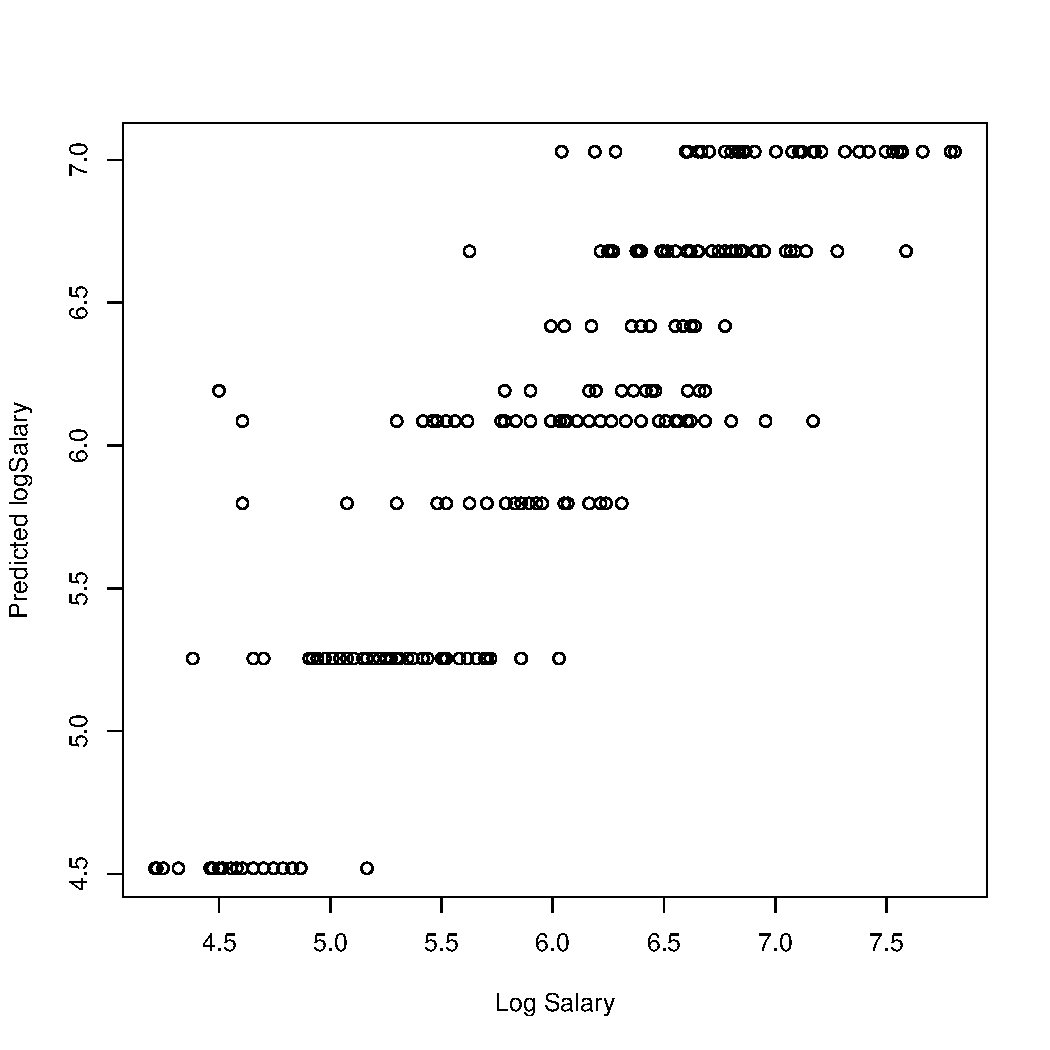
\includegraphics[width=0.6\textwidth]{figure/unnamed-chunk-6-1} 

}



\end{knitrout}

Questions:
\begin{enumerate}
  \item What is going on in this plot? Do these patterns in the prediction make sense? If yes, why do they make sense?
  \item Recalling output in handout 4.1.1, what do the ``important'' variables have in common?
\end{enumerate}

\newpage

\subsection*{Random Forests}

\begin{knitrout}
\definecolor{shadecolor}{rgb}{0.969, 0.969, 0.969}\color{fgcolor}\begin{kframe}
\begin{alltt}
\hlcom{# Set a seed for reproducibility}
\hlkwd{set.seed}\hlstd{(}\hlnum{10984}\hlstd{)}

\hlcom{# For the random forest to be trained correctly, we must handle the 118}
\hlcom{# missing values in the baseball dataset. Correctly handling NA values is an}
\hlcom{# incredibly deep topic, but for the sake of simplicity we will simply just}
\hlcom{# remove all rows from the baseball dataframe that have missing values.}
\hlstd{baseball} \hlkwb{<-} \hlkwd{na.omit}\hlstd{(baseball)}

\hlcom{# Train a random forest model}
\hlstd{baseball_rf} \hlkwb{<-}
  \hlstd{randomForest}\hlopt{::}\hlkwd{randomForest}\hlstd{(logSalary} \hlopt{~} \hlstd{nAtBat} \hlopt{+} \hlstd{nHits} \hlopt{+} \hlstd{nHome} \hlopt{+} \hlstd{nRuns} \hlopt{+} \hlstd{nRBI} \hlopt{+}
                               \hlstd{nBB} \hlopt{+} \hlstd{YrMajor} \hlopt{+} \hlstd{CrAtBat} \hlopt{+} \hlstd{CrHits} \hlopt{+} \hlstd{CrHome} \hlopt{+}
                               \hlstd{CrRuns} \hlopt{+} \hlstd{CrRbi} \hlopt{+} \hlstd{CrBB} \hlopt{+} \hlstd{League} \hlopt{+} \hlstd{Division} \hlopt{+}
                               \hlstd{nOuts} \hlopt{+} \hlstd{nAssts} \hlopt{+} \hlstd{nError,} \hlkwc{data} \hlstd{= baseball)}

\hlcom{# Check out a variable importance plot of the random forest:}
\hlstd{randomForest}\hlopt{::}\hlkwd{varImpPlot}\hlstd{(baseball_rf)}
\end{alltt}
\end{kframe}

{\centering 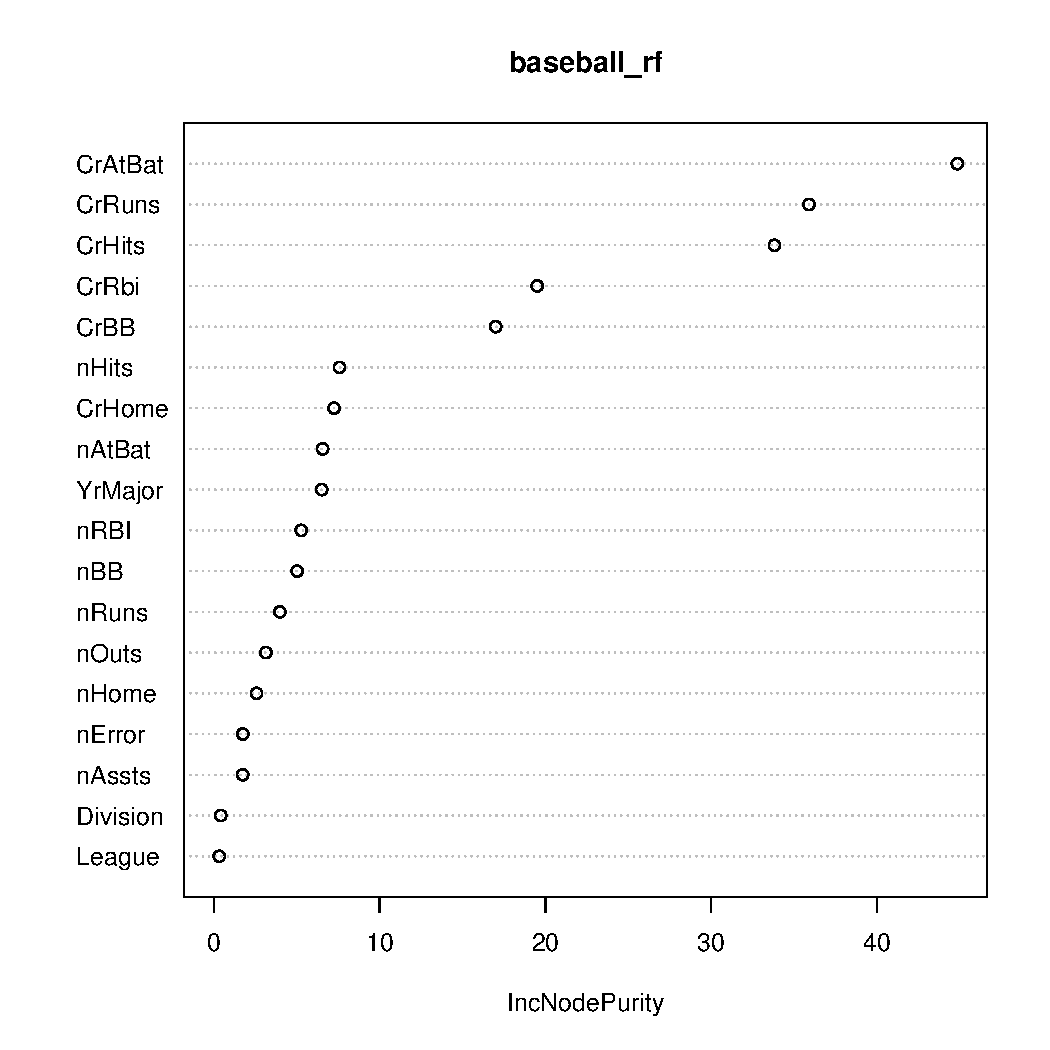
\includegraphics[width=0.6\textwidth]{figure/unnamed-chunk-7-1} 

}



\end{knitrout}


\end{document}
